% Options for packages loaded elsewhere
\PassOptionsToPackage{unicode}{hyperref}
\PassOptionsToPackage{hyphens}{url}
\documentclass[
  11pt,
]{article}
\usepackage{xcolor}
\usepackage[left=3cm,right=3cm,top=2.5cm,bottom=2.5cm]{geometry}
\usepackage{amsmath,amssymb}
\setcounter{secnumdepth}{5}
\usepackage{iftex}
\ifPDFTeX
  \usepackage[T1]{fontenc}
  \usepackage[utf8]{inputenc}
  \usepackage{textcomp} % provide euro and other symbols
\else % if luatex or xetex
  \usepackage{unicode-math} % this also loads fontspec
  \defaultfontfeatures{Scale=MatchLowercase}
  \defaultfontfeatures[\rmfamily]{Ligatures=TeX,Scale=1}
\fi
\usepackage{lmodern}
\ifPDFTeX\else
  % xetex/luatex font selection
\fi
% Use upquote if available, for straight quotes in verbatim environments
\IfFileExists{upquote.sty}{\usepackage{upquote}}{}
\IfFileExists{microtype.sty}{% use microtype if available
  \usepackage[]{microtype}
  \UseMicrotypeSet[protrusion]{basicmath} % disable protrusion for tt fonts
}{}
\usepackage{setspace}
\makeatletter
\@ifundefined{KOMAClassName}{% if non-KOMA class
  \IfFileExists{parskip.sty}{%
    \usepackage{parskip}
  }{% else
    \setlength{\parindent}{0pt}
    \setlength{\parskip}{6pt plus 2pt minus 1pt}}
}{% if KOMA class
  \KOMAoptions{parskip=half}}
\makeatother
\usepackage{longtable,booktabs,array}
\usepackage{caption}
\captionsetup[table]{skip=6pt}
\newcounter{none} % for unnumbered tables
\usepackage{calc} % for calculating minipage widths
% Correct order of tables after \paragraph or \subparagraph
\usepackage{etoolbox}
\makeatletter
\patchcmd\longtable{\par}{\if@noskipsec\mbox{}\fi\par}{}{}
\makeatother
% Allow footnotes in longtable head/foot
\IfFileExists{footnotehyper.sty}{\usepackage{footnotehyper}}{\usepackage{footnote}}
\makesavenoteenv{longtable}
\usepackage{graphicx}
\makeatletter
\newsavebox\pandoc@box
\newcommand*\pandocbounded[1]{% scales image to fit in text height/width
  \sbox\pandoc@box{#1}%
  \Gscale@div\@tempa{\textheight}{\dimexpr\ht\pandoc@box+\dp\pandoc@box\relax}%
  \Gscale@div\@tempb{\linewidth}{\wd\pandoc@box}%
  \ifdim\@tempb\p@<\@tempa\p@\let\@tempa\@tempb\fi% select the smaller of both
  \ifdim\@tempa\p@<\p@\scalebox{\@tempa}{\usebox\pandoc@box}%
  \else\usebox{\pandoc@box}%
  \fi%
}
% Set default figure placement to htbp
\def\fps@figure{htbp}
\makeatother
% definitions for citeproc citations
\NewDocumentCommand\citeproctext{}{}
\NewDocumentCommand\citeproc{mm}{%
  \begingroup\def\citeproctext{#2}\cite{#1}\endgroup}
\makeatletter
 % allow citations to break across lines
 \let\@cite@ofmt\@firstofone
 % avoid brackets around text for \cite:
 \def\@biblabel#1{}
 \def\@cite#1#2{{#1\if@tempswa , #2\fi}}
\makeatother
\newlength{\cslhangindent}
\setlength{\cslhangindent}{1.5em}
\newlength{\csllabelwidth}
\setlength{\csllabelwidth}{3em}
\newenvironment{CSLReferences}[2] % #1 hanging-indent, #2 entry-spacing
 {\begin{list}{}{%
  \setlength{\itemindent}{0pt}
  \setlength{\leftmargin}{0pt}
  \setlength{\parsep}{0pt}
  % turn on hanging indent if param 1 is 1
  \ifodd #1
   \setlength{\leftmargin}{\cslhangindent}
   \setlength{\itemindent}{-1\cslhangindent}
  \fi
  % set entry spacing
  \setlength{\itemsep}{#2\baselineskip}}}
 {\end{list}}
\usepackage{calc}
\newcommand{\CSLBlock}[1]{\hfill\break\parbox[t]{\linewidth}{\strut\ignorespaces#1\strut}}
\newcommand{\CSLLeftMargin}[1]{\parbox[t]{\csllabelwidth}{\strut#1\strut}}
\newcommand{\CSLRightInline}[1]{\parbox[t]{\linewidth - \csllabelwidth}{\strut#1\strut}}
\newcommand{\CSLIndent}[1]{\hspace{\cslhangindent}#1}
\setlength{\emergencystretch}{3em} % prevent overfull lines
\providecommand{\tightlist}{%
  \setlength{\itemsep}{0pt}\setlength{\parskip}{0pt}}
%% tools/stamp.tex
%% Provenance footer for PDFs rendered from this project.
%% Vendored by zzcollab; this file is not project-specific. The
%% footer prints the source document and the time of rendering.
%% The git version is defined here too, and so is available to a
%% project that wants it on the page, but it is left off the
%% default footer: it already names the staged copy in share/ and
%% appears in its manifest row. All values are supplied at render
%% time by tools/stamp-render.R, which writes a small generated
%% file that redefines the macros below. The \providecommand
%% defaults keep a bare LaTeX compile working when the document is
%% built without the wrapper.
\usepackage{fancyhdr}
\usepackage{xcolor}
\providecommand{\stampsource}{\detokenize{(source not recorded)}}
\providecommand{\stamptime}{(time not recorded)}
\providecommand{\stampversion}{\detokenize{(version not recorded)}}
\setlength{\footskip}{40pt}
\newcommand{\stampfootcontent}{%
  \footnotesize\color{gray}%
  \parbox[b]{\textwidth}{%
    \stamptime\hfill\thepage\\[2pt]%
    \ttfamily\raggedright\stampsource}}
\pagestyle{fancy}
\fancyhf{}
\fancyfoot[C]{\stampfootcontent}
\renewcommand{\headrulewidth}{0pt}
\renewcommand{\footrulewidth}{0.4pt}
%% The title page uses the `plain` page style; redefine it so the
%% stamp appears there too.
\fancypagestyle{plain}{%
  \fancyhf{}%
  \fancyfoot[C]{\stampfootcontent}%
  \renewcommand{\headrulewidth}{0pt}%
  \renewcommand{\footrulewidth}{0.4pt}}
\renewcommand{\stampsource}{\textasciitilde{}/\allowbreak{}prj/\allowbreak{}res/\allowbreak{}05-optimal-visit-placement/\allowbreak{}visitplacement/\allowbreak{}analysis/\allowbreak{}report/\allowbreak{}report.Rmd}
\renewcommand{\stamptime}{2026-08-20 14:03 PDT}
\renewcommand{\stampversion}{\detokenize{6717595-wip}}
\usepackage{amsmath}
\usepackage{amssymb}
\usepackage{booktabs}
\usepackage{longtable}
\usepackage{float}
\usepackage[mathlines]{lineno}
\linenumbers
\usepackage{booktabs}
\usepackage{longtable}
\usepackage{array}
\usepackage{multirow}
\usepackage{wrapfig}
\usepackage{float}
\usepackage{colortbl}
\usepackage{pdflscape}
\usepackage{tabu}
\usepackage{threeparttable}
\usepackage{threeparttablex}
\usepackage[normalem]{ulem}
\usepackage{makecell}
\usepackage{xcolor}
\usepackage{bookmark}
\IfFileExists{xurl.sty}{\usepackage{xurl}}{} % add URL line breaks if available
\urlstyle{same}
% fallback for those not using the hyperref driver hyperxmp:
\makeatletter
\@ifundefined{xmpquote}{\newcommand{\xmpquote}[1]{#1}}{}
\makeatother
\hypersetup{
  pdftitle={Efficiency Consequences of Visit Schedule Choice in Longitudinal Trials: An Analytic and Simulation-Based Comparison},
  pdfauthor={Ronald G. Thomas, Ph.D.},
  pdfkeywords={\xmpquote{longitudinal data; optimal design; visit schedule; linear mixed model; Monte Carlo simulation; relative efficiency}},
  hidelinks,
  pdfcreator={LaTeX via pandoc}}

\title{Efficiency Consequences of Visit Schedule Choice in Longitudinal Trials: An Analytic and Simulation-Based Comparison}
\author{Ronald G. Thomas, Ph.D.\thanks{Wertheim School of Public Health, UCSD; ORCID: 0000-0003-1686-4965}}
\date{August 20, 2026}

\begin{document}
\maketitle
\begin{abstract}
Observation times in longitudinal clinical trials are usually
spaced equally for administrative convenience, but optimal design
theory shows that placement affects the precision of estimated
treatment effects. We compare an equally spaced five-visit
schedule with a boundary-clustered schedule for a two-arm,
24-month trial with a linearly divergent treatment effect,
combining an exact generalized least squares (GLS) efficiency
calculation with a common-random-number Monte Carlo study (2000
paired replications) under a random-intercept, random-slope data
generating model. The analytic relative efficiency of the
clustered design is 1.06, and the paired simulation, after
recalibrating the effect size so power is informative rather than
at ceiling, reproduces this result (empirical relative efficiency
1.07, 95\% bootstrap interval 1.06-1.09), confirming that the
precision advantage is real and not simulation noise. We do not
claim optimality: the theoretically optimal design for this
covariance structure is not computed here, and only two designs
are compared. The contribution is a worked, fully reproducible
demonstration of how much efficiency is at stake for one realistic
configuration, and a template (\texttt{R/simulation.R}) for extending the
comparison to other covariance structures, dropout mechanisms, and
candidate schedules.
\end{abstract}

{
\setcounter{tocdepth}{2}
\tableofcontents
}
\setstretch{1.1}
\section{Introduction}\label{introduction}

In longitudinal clinical trials, subjects are measured
repeatedly over a fixed study period. The conventional approach
assigns observation times at equally spaced intervals (monthly
or quarterly visits, for example) largely for administrative
convenience rather than statistical efficiency. A growing body
of work in optimal experimental design suggests that the
placement of these observation times can substantially affect
the precision with which treatment effects are estimated. We
begin in Section \ref{optimal-allocation-of-observation-times}
with a review of the relevant literature and then describe the
analytic efficiency calculation and simulation study, and their
results, in Sections \ref{methods} and \ref{results}.

\subsection{Optimal allocation of observation times}\label{optimal-allocation-of-observation-times}

\textsuperscript{\citeproc{ref-winkensOptimalTimepointsClinical2005}{1}} provided the foundational
analysis of this problem for two-group trials with linearly
divergent treatment effects. They showed that the optimal
allocation of time-points depends critically on the assumed
covariance structure. Under compound symmetry (CS), efficiency
improves by clustering repeated measures near the end of the
study period, where the treatment effect is largest. Under a
first-order autoregressive (AR(1)) structure, only two
measurements -- at baseline and at study end -- are needed for
highly efficient estimation. Under a more realistic AR(1) plus
measurement error structure, the optimal spacing depends on the
specific covariance parameter values, but the equally spaced
design is generally suboptimal.

In a companion paper,\textsuperscript{\citeproc{ref-winkensOptimalNumberRepeated2006}{2}} extended
these results to address the joint optimization of the number
of repeated measures and group sizes under budget constraints.
They found that when budget is fixed and the covariance structure
includes an autoregressive component, two repeated measures per
subject often yield highly efficient treatment effect estimators.
Otherwise, intermediate measures can reduce the variance of the
generalized least squares (GLS) estimator, particularly under
compound symmetry.

\subsection{Design criteria and cost considerations}\label{design-criteria-and-cost-considerations}

The formal framework for these results relies on classical
optimal design theory, as developed by\textsuperscript{\citeproc{ref-atkinson1992optimum}{3}}.\textsuperscript{\citeproc{ref-ouwens2002maximin}{4}} proposed maximin D-optimal designs for
longitudinal mixed effects models, computing optimal allocations
of time-points for polynomial trend models with random
intercepts, random slopes, and AR(1) serial correlations. Because
D-optimal designs depend on unknown parameter values, the
maximin criterion provides robustness by maximizing the worst-case
relative efficiency across the parameter space.

\textsuperscript{\citeproc{ref-tekle2008doptimal}{5}} extended this work to cohort designs, showing
that a purely longitudinal design with a single cohort measured
at optimal time-points is generally more efficient than mixed
longitudinal-cross-sectional designs. Their numerical results
demonstrated that the most efficient number of repeated
measurements equals the sum of the number of cohorts and the
degree of the polynomial trend. Subsequently,\textsuperscript{\citeproc{ref-tekle2011cohorts}{6}} showed that adding cohorts or repeated
measurements beyond this optimum wastes resources when the study
budget is fixed.

\subsection{Practical guidance on the number of measures}\label{practical-guidance-on-the-number-of-measures}

From a more pragmatic perspective,\textsuperscript{\citeproc{ref-vickers2003howmany}{7}} examined
the marginal benefit of adding repeated measures in terms of
statistical power. He showed that while repeating assessments
can have dramatic effects on power, the marginal benefit of each
additional measure decreases rapidly. In general, there is little value in exceeding four
post-treatment assessments (or seven total including baseline),
except when correlations between measures are low, as in
episodic conditions.

\subsection{Extensions and related work}\label{extensions-and-related-work}

Several extensions of the Winkens framework have appeared.\textsuperscript{\citeproc{ref-winkens2007polynomial}{8}} generalized the optimal design results to
second-order polynomial treatment effects, finding that equidistant
time-points are either optimal or highly efficient when only three
measures are taken.\textsuperscript{\citeproc{ref-candel2008empirical}{9}} investigated optimal
designs when the goal is to estimate individual growth curves
(random effects) rather than fixed effects, showing that the
optimal number of time-points and subjects differs from the
fixed-effects case.\textsuperscript{\citeproc{ref-abebe2014bayesian}{10}} developed Bayesian
D-optimal designs for dichotomous repeated measures with
autocorrelation, formally accounting for parameter uncertainty
through prior distributions.

For the analysis of unequally spaced longitudinal data,\textsuperscript{\citeproc{ref-jones1991unequally}{11}} provided the statistical machinery for
fitting mixed models with continuous-time AR(1) structures and
arbitrary observation schedules. Their approach, based on the
Kalman filter, remains foundational for analyzing data from
designs with non-equidistant time-points.

\subsection{Power and sample size tools}\label{power-and-sample-size-tools}

Modern software for power and sample size calculations in
longitudinal trials has made these design considerations more
accessible.\textsuperscript{\citeproc{ref-iddi2022longpower}{12}} describe the \texttt{longpower} R
package, which implements closed-form power calculations for
linear mixed models.\textsuperscript{\citeproc{ref-donohue2010power}{13}} applied these methods
to Alzheimer's disease Phase II trial design, demonstrating
the practical impact of design choices on the ability to detect
disease-modifying treatment effects.

\subsection{Present study}\label{present-study}

The theoretical optimality results reviewed above establish that
the best design depends on the assumed covariance structure, but
they do not by themselves quantify how much efficiency is at
stake for a specific, realistic trial configuration, nor do they
address the finite-sample behavior of the REML-based inference
that practitioners actually use. This report addresses that
translational gap for one configuration: a 100-patient, two-arm,
24-month trial with a linearly divergent treatment effect,
analyzed under a random-intercept, random-slope model. We compare
two five-visit designs:

\begin{itemize}
\tightlist
\item
  \textbf{Equal spacing:} observations at months 0, 6, 12, 18, and 24.
\item
  \textbf{Clustered spacing:} observations clustered near the
  beginning and end of the study period (months 0, 2, 4, 20, 24).
  Under a random-slope covariance structure (Section
  \ref{data-generating-model}), boundary-loaded time-points are
  efficient for estimating the slope contrast for a classical
  leverage reason -- observations far from the mean time carry more
  information about a slope -- which is distinct from the
  compound-symmetry mechanism that motivates clustering in\textsuperscript{\citeproc{ref-winkensOptimalTimepointsClinical2005}{1}}; see Section
  \ref{covariance-structure-and-theoretical-prediction} for the
  derivation.
\end{itemize}

We first derive the exact asymptotic (GLS) relative efficiency of
the two designs in closed form, then use a common-random-number
Monte Carlo study to assess whether finite-sample REML estimation
and inference (bias, empirical versus model-based standard error,
power, and 95\% confidence interval coverage) reproduce the
analytic prediction. We do not claim that either design is
optimal: the theoretically optimal design implied by the cited
literature is not computed here, and only two candidate schedules
are compared. \texttt{R/simulation.R} in the accompanying compendium
implements the data-generating model, the analytic efficiency
calculation, and the paired simulation as reusable functions so
the comparison can be extended to other covariance structures,
sample sizes, dropout mechanisms, and candidate schedules (Section
\ref{scenario-extension-analytic-only}).

\section{Methods}\label{methods}

\subsection{Data generating model}\label{data-generating-model}

We simulate data from a linear mixed effects model with random
intercepts and random slopes. Let \(Y_{ij}\) denote the outcome for
subject \(i\) at time \(t_j\). The generating model is:

\[
Y_{ij} = (\beta_0 + b_{0i}) +
         (\beta_1 + b_{1i}) \, t_j +
         \beta_2 \, G_i +
         \beta_3 \, G_i \, t_j +
         \varepsilon_{ij}
\]

where \(G_i \in \{0, 1\}\) is the treatment group indicator,
\(b_{0i}\) and \(b_{1i}\) are subject-specific random effects
with \(\text{Var}(b_0) = \tau_0^2\), \(\text{Var}(b_1) = \tau_1^2\),
\(\text{Cov}(b_0, b_1) = \tau_{01}\), and
\(\varepsilon_{ij} \sim N(0, \sigma^2)\).

The parameter of interest is \(\beta_3\), the treatment-by-time
interaction, which represents the rate at which the treatment
effect diverges from the control effect per unit time.

\subsection{Covariance structure and theoretical prediction}\label{covariance-structure-and-theoretical-prediction}

Marginalizing over the random effects, this model induces a
within-subject covariance
\(\text{Cov}(Y_{ij}, Y_{ij'}) = \tau_0^2 + \tau_{01}(t_j + t_{j'}) +
\tau_1^2 t_j t_{j'} + \sigma^2 \mathbb{1}(j = j')\), in which the
marginal variance increases with \(t_j^2\) and the correlation
between visits depends on their product \(t_j t_{j'}\), not on their
lag \(|t_j - t_{j'}|\). This is the standard random-coefficients
(random-intercept, random-slope) covariance structure. It is
distinct from both compound symmetry (CS), which is the
random-intercept-only special case (\(\tau_1 = 0\)) with constant
correlation regardless of visit timing, and from a first-order
autoregressive (AR(1)) structure, whose correlation depends only on
the lag between visits and does not grow with \(\tau_1\) boundary
leverage. An earlier draft of this report described the simulated
structure as combining features of CS and AR(1); that
characterization is incorrect and has been removed (see the
Discussion for the corrected interpretation).

The efficiency prediction relevant to this structure differs from
the CS-based argument in\textsuperscript{\citeproc{ref-winkensOptimalTimepointsClinical2005}{1}}.
Under CS, clustering observations near the end of the study helps
because the treatment effect (and hence the signal) is largest
there while every pair of visits is equally correlated, so nothing
is lost by leaving a gap. Under the random-slope structure
simulated here, the reason boundary-clustered designs are more
efficient for the \emph{slope} contrast \(\beta_3\) is instead the
classical leverage argument for regression slopes: for a simple
linear regression of \(Y\) on \(t\), \(\text{Var}(\hat{\text{slope}})
\propto 1 / \sum_i (t_i - \bar{t})^2\), so observations placed far
from the mean time carry disproportionately more information about
the slope. Section \ref{analytic-relative-efficiency} below
verifies this prediction is directionally correct but shows the
efficiency gain shrinks as the random-slope variance \(\tau_1^2\)
grows relative to the residual variance, because a larger
\(\tau_1^2\) makes the slope itself (not just its estimation error)
more variable across subjects, which increases the total variance
contributed by every visit and dilutes the boundary-leverage
advantage.

\subsection{Parameter values}\label{parameter-values}

We use the following parameter values, broadly motivated by
cognitive decline trials:

\begin{table}[!h]
\centering
\caption{\label{tab:params}Simulation parameters.}
\centering
\fontsize{10}{12}\selectfont
\begin{tabular}[t]{llr}
\toprule
Parameter & Symbol & Value\\
\midrule
Intercept & $\beta_0$ & 50.00\\
Time slope & $\beta_1$ & -1.00\\
Group effect at baseline & $\beta_2$ & 0.00\\
Group x time & $\beta_3$ & 0.19\\
SD random intercept & $\tau_0$ & 5.00\\
\addlinespace
SD random slope & $\tau_1$ & 0.30\\
Residual SD & $\sigma$ & 3.00\\
Subjects per group & $n$ & 50.00\\
Study duration (months) & -- & 24.00\\
Number of simulations & -- & 2000.00\\
\bottomrule
\end{tabular}
\end{table}

The treatment-by-time interaction \(\beta_3 = 0.19\) implies that
the treatment group improves (or declines less) by 0.19 units per
month relative to control, yielding a cumulative treatment
advantage of 4.56 units over 24
months.

\subsubsection{Recalibration of the treatment effect}\label{recalibration-of-the-treatment-effect}

An earlier draft used \(\beta_3 = 0.5\), for which the analytic power
of both designs is 1 to machine precision (Section
\ref{analytic-relative-efficiency}): every replication rejects the
null, so power cannot discriminate between designs and the metric
is uninformative. We recalibrated \(\beta_3\) so that the
equal-spacing design has approximately 80\% analytic power at the
two-sided \(\alpha = 0.05\) level, which requires
\(\beta_3 / \text{SE}_{\text{equal}} \approx 2.80\) (the sum of the
\(z\)-quantiles for 80\% power and a two-sided 5\% test). With
\(\text{SE}_{\text{equal}} = 0.0678\) (Section
\ref{analytic-relative-efficiency}), this gives \(\beta_3 \approx
0.19\), for which the analytic power is 80.0\% (equal spacing) and
82.4\% (clustered spacing) -- close to, and not at, the ceiling, so
that power remains informative while both designs are still
adequately powered for a realistic trial. All other parameters are
unchanged from the original design.

\subsection{Design specifications}\label{design-specifications}

\begin{table}[!h]
\centering
\caption{\label{tab:design-table}Observation times (months) for each design.}
\centering
\fontsize{10}{12}\selectfont
\begin{tabular}[t]{lrrrrr}
\toprule
Design & Visit 1 & Visit 2 & Visit 3 & Visit 4 & Visit 5\\
\midrule
Equal & 0 & 6 & 12 & 18 & 24\\
Clustered & 0 & 2 & 4 & 20 & 24\\
\bottomrule
\end{tabular}
\end{table}

\begin{figure}

{\centering 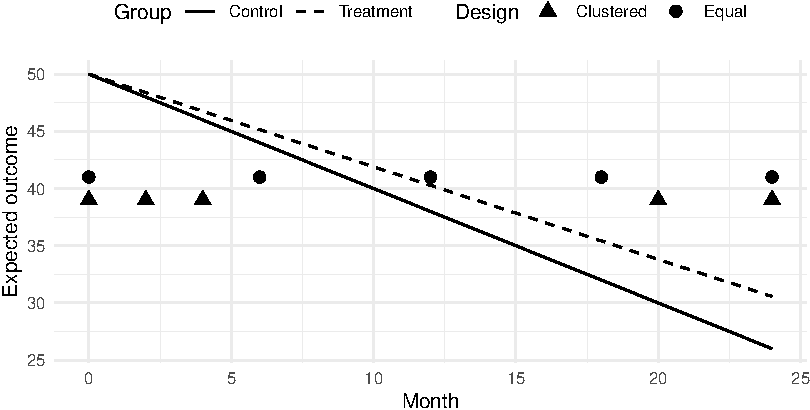
\includegraphics{report_files/figure-latex/design-visual-1} 

}

\caption{Schematic of the two visit schedules over the 24-month study period. Lines show the expected group trajectories; markers show each design's visit times, vertically offset (Equal above, Clustered below) purely to avoid overplotting at shared visit times (0 and 24 months) and carry no other meaning.}\label{fig:design-visual}
\end{figure}

\subsection{Analytic relative efficiency}\label{analytic-relative-efficiency}

Under the data generating model of Section
\ref{data-generating-model}, the treatment-by-time interaction
\(\hat{\beta}_3\) has an exact large-sample GLS variance: with
\(\mathbf{Z}_i = [\mathbf{1}, \mathbf{t}]\) the \(k \times 2\) per-subject
design matrix for the random effects, \(\mathbf{D}\) the random-effects
covariance matrix, and
\(\mathbf{V} = \mathbf{Z}_i \mathbf{D} \mathbf{Z}_i' + \sigma^2
\mathbf{I}_k\), the information matrix
\(\mathbf{M} = \sum_i \mathbf{X}_i' \mathbf{V}^{-1} \mathbf{X}_i\)
(summed separately over control subjects, for whom the last two
columns of \(\mathbf{X}_i\) are zero, and treatment subjects) gives
\(\text{Var}(\hat{\beta}_3) = [\mathbf{M}^{-1}]_{44}\). This ten-line
linear algebra calculation, implemented as \texttt{analytic\_gls\_se()} in
\texttt{R/simulation.R}, requires no simulation:

\begin{table}[!h]
\centering
\caption{\label{tab:analytic-efficiency}Exact GLS standard errors of the treatment-by-time interaction under the random-slope data-generating model.}
\centering
\fontsize{10}{12}\selectfont
\begin{tabular}[t]{lr}
\toprule
Design & Analytic SE\\
\midrule
Equal & 0.0678\\
Clustered & 0.0658\\
\bottomrule
\end{tabular}
\end{table}

The exact GLS standard errors are
0.0678 (equal spacing) and
0.0658 (clustered spacing),
giving a relative efficiency (ratio of variances) of
1.063 in favor of the clustered design.
This analytic value is the primary quantity of interest for the
design comparison; the simulation in Section
\ref{simulation-procedure} exists to answer a different question --
whether finite-sample REML estimation and Wald-type inference
(bias, coverage, and empirical versus model-based SE) reproduce
this analytic prediction and behave as expected at \(n = 100\) -- not
to re-derive a number already available in closed form.

\subsection{Scenario extension (analytic only)}\label{scenario-extension-analytic-only}

The single scenario simulated in this report fixes one covariance
structure, one effect size, and one sample size (2026-08-16
review, issue 2.4). Because the design comparison's quantity of
interest, the GLS relative efficiency, has a closed form (Section
\ref{analytic-relative-efficiency}), \texttt{analytic\_gls\_se\_general()}
in \texttt{R/covariance.R} generalizes the calculation to an arbitrary
within-subject covariance matrix, so the sensitivity of the
efficiency contrast to the covariance structure can be assessed
without additional Monte Carlo simulation. Table
\ref{tab:scenario-grid} reports the exact relative efficiency of
the clustered versus equal-spacing design across the random-slope
SD \(\tau_1\) used in the main simulation, and for two additional
structures: compound symmetry, the mechanism that motivates
clustering in\textsuperscript{\citeproc{ref-winkensOptimalTimepointsClinical2005}{1}}, and AR(1)
plus measurement error.

\begin{table}[!h]
\centering
\caption{\label{tab:scenario-grid}Analytic (closed-form, no simulation) relative efficiency of the clustered versus equal-spacing design across covariance structures and random-slope variance.}
\centering
\fontsize{9}{11}\selectfont
\begin{tabular}[t]{llrrr}
\toprule
Structure & Parameter & SE (Equal) & SE (Clustered) & Relative efficiency\\
\midrule
Random slope & tau\_1 = 0.10 & 0.0374 & 0.0336 & 1.24\\
Random slope & tau\_1 = 0.20 & 0.0510 & 0.0482 & 1.12\\
Random slope & tau\_1 = 0.30 & 0.0678 & 0.0658 & 1.06\\
Random slope & tau\_1 = 0.40 & 0.0860 & 0.0844 & 1.04\\
Random slope & tau\_1 = 0.50 & 0.1049 & 0.1036 & 1.03\\
\addlinespace
Compound symmetry & tau\_0 = 5.0 & 0.0316 & 0.0269 & 1.38\\
AR(1) + error & rho = 0.8 & 0.0554 & 0.0528 & 1.10\\
\bottomrule
\end{tabular}
\end{table}

The clustered design is more efficient across the full
random-slope grid, but the advantage shrinks as \(\tau_1\) grows
relative to the residual SD \(\sigma\), consistent with the
leverage-dilution argument of Section
\ref{covariance-structure-and-theoretical-prediction}. Under
compound symmetry and under AR(1) plus measurement error the
clustered design is also more efficient, although by a different
mechanism in each case. This extension is analytic only: it does
not assess whether finite-sample REML estimation and inference
reproduce these predictions for structures other than the
random-slope structure actually simulated, nor does it vary
sample size or dropout. Extending the Monte Carlo comparison
itself to this grid, and to dropout, remains future work (see the
Discussion); \texttt{Rscript\ analysis/scripts/run\_scenario\_grid.R}
regenerates Table \ref{tab:scenario-grid}.

\subsection{Simulation procedure}\label{simulation-procedure}

The simulation functions (\texttt{simulate\_trial()}, \texttt{run\_one\_sim()},
\texttt{run\_paired\_simulation()}, \texttt{analytic\_gls\_se()}) live in \texttt{R/} as
documented, unit-tested package functions (\texttt{inst/tinytest/}) rather
than inline in this document, so they can be reused for the
scenario extension and audited independently of the manuscript
(2026-08-16 review, issue 2.8). For each of 2000 Monte Carlo
replications, \texttt{run\_paired\_simulation()}:

\begin{enumerate}
\def\labelenumi{\arabic{enumi}.}
\tightlist
\item
  Generates 100 subjects, randomized 1:1 to treatment
  and control, drawing one shared set of subject-level random
  effects \((b_{0i}, b_{1i})\) and one shared set of residual errors
  \(\varepsilon_{ij}\) per subject-visit index \(j = 1, \dots, 5\).
\item
  Builds the equal-spacing and clustered-spacing datasets from
  \emph{those same draws}, so the \(j\)-th random effect and residual
  realization is reused across designs for the \(j\)-th visit rather
  than redrawn -- these are common random numbers (CRN), which
  pair the two designs within each replication and substantially
  reduce the Monte Carlo error of the \emph{difference} between designs
  relative to two independent simulation arms.
\item
  Fits a linear mixed model (random intercepts and slopes) to each
  design's dataset using restricted maximum likelihood (REML) via
  \texttt{nlme::lme()}.
\item
  Extracts the point estimate, standard error, and \(p\)-value for
  \(\hat{\beta}_3\) for each design.
\end{enumerate}

For each design we compute the mean estimate (bias), the empirical
SD of \(\hat{\beta}_3\), the mean model-based SE, empirical power
(\(p < 0.05\)), and 95\% CI coverage, each with a Monte Carlo standard
error (MCSE) computed following\textsuperscript{\citeproc{ref-morris2019simulation}{14}}: MCSE of the
empirical SD is \(\text{SE} / \sqrt{2(R-1)}\), MCSE of a proportion
(power, coverage) is \(\sqrt{\hat p (1-\hat p) / R}\), and MCSE of the
bias is \(\text{SE} / \sqrt{R}\), where \(R\) is the number of converged
replications. We additionally report a paired bootstrap (resampling
replication indices, which respects the CRN pairing) 95\% interval
for the relative efficiency (ratio of empirical variances).

The driver script \texttt{analysis/scripts/run\_simulation.R} runs this
procedure and saves the raw per-replication estimates, the summary
statistics with MCSEs, the analytic SEs, and the bootstrap interval
to a single versioned artifact,
\texttt{analysis/data/derived\_data/sim\_results.rds}, which this document
reads directly rather than re-simulating on every render or relying
on the knitr cache to stay synchronized with the reported numbers
(2026-08-16 review, issue 2.8(e)). To regenerate:
\texttt{Rscript\ analysis/scripts/run\_simulation.R\ 2000}. The results below
used 2000 replications, R version 4.6.1 (2026-06-24),
and \texttt{nlme} 3.1.169, completing in
176 seconds
(single core, no parallelization).

\section{Results}\label{results}

\subsection{Summary statistics}\label{summary-statistics}

\begin{table}[!h]
\centering
\caption{\label{tab:summary-table}Simulation results for the treatment-by-time interaction, with Monte Carlo standard errors (MCSE) of each metric computed following Morris, White, and Crowther (2019).}
\centering
\resizebox{\ifdim\width>\linewidth\linewidth\else\width\fi}{!}{
\fontsize{8}{10}\selectfont
\begin{tabular}[t]{lrrrrrrrrrrr}
\toprule
Design & Converged & Mean Est. & Bias & MCSE(Bias) & Emp. SE & MCSE(Emp. SE) & Model SE & Power & MCSE(Power) & Coverage & MCSE(Coverage)\\
\midrule
Equal & 2000 & 0.189 & -0.0011 & 0.0015 & 0.0669 & 0.0011 & 0.0676 & 0.787 & 0.0092 & 0.952 & 0.0048\\
Clustered & 2000 & 0.189 & -0.0015 & 0.0014 & 0.0646 & 0.0010 & 0.0655 & 0.814 & 0.0087 & 0.957 & 0.0046\\
\bottomrule
\end{tabular}}
\end{table}

Replications for which \texttt{nlme::lme()} failed to converge (an
error or warning during fitting, per \texttt{run\_one\_sim()} in
\texttt{R/simulation.R}) are recorded as \texttt{NA} and excluded from the
summary statistics above rather than imputed or retried; the
\texttt{Converged} column reports how many of the 2000 attempted
replications per design contributed to each summary statistic.

We observe that the equal-spacing design achieves an empirical
power of 78.7\% (MCSE 0.9\%), compared with 81.3\% (MCSE
0.9\%) for the
clustered design; both are informative rather than at ceiling
following the recalibration of \(\beta_3\) (Section
\ref{recalibration-of-the-treatment-effect}). The empirical
standard error of \(\hat{\beta}_3\) is 0.0669 (MCSE
0.00106) under equal spacing and
0.0646 (MCSE 0.00102) under
the clustered design. The paired-bootstrap relative efficiency (ratio
of empirical variances, resampling replication indices so the
common-random-number pairing is respected) is 1.07, 95\% bootstrap interval 1.06-1.09, consistent
with the analytic relative efficiency of 1.063 (Section \ref{analytic-relative-efficiency}); the
interval excludes 1, so the precision advantage of the clustered
design is distinguishable from Monte Carlo noise.

\subsection{Distribution of estimates}\label{distribution-of-estimates}

\begin{figure}

{\centering 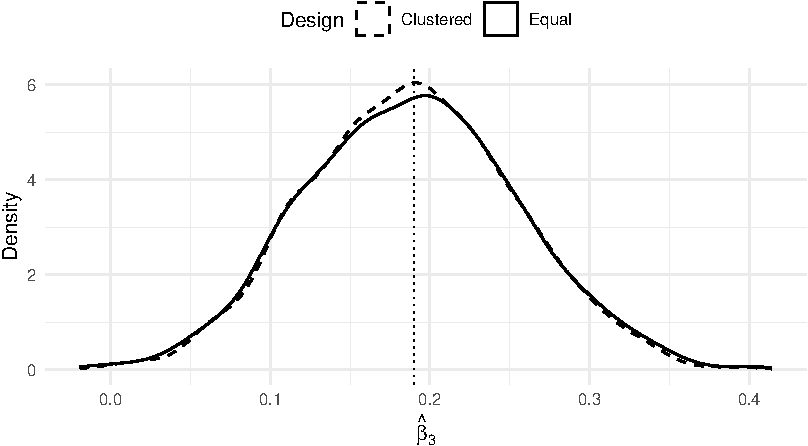
\includegraphics{report_files/figure-latex/density-plot-1} 

}

\caption{Sampling distribution of the treatment-by-time interaction estimate under each design.}\label{fig:density-plot}
\end{figure}

\subsection{Standard errors across simulations}\label{standard-errors-across-simulations}

\begin{figure}

{\centering 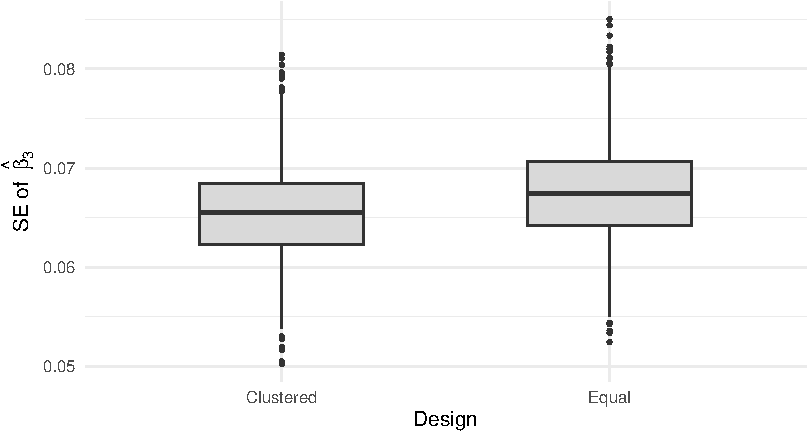
\includegraphics{report_files/figure-latex/se-boxplot-1} 

}

\caption{Distribution of model-based standard errors across simulations.}\label{fig:se-boxplot}
\end{figure}

\section{Discussion}\label{discussion}

In this study, we have endeavored to illustrate the practical
consequences of visit placement in longitudinal clinical trials.
Both designs use the same number of subjects and the same number
of visits; they differ only in the timing of observations.

The results are broadly consistent, in direction, with the
theoretical findings of\textsuperscript{\citeproc{ref-winkensOptimalTimepointsClinical2005}{1}},
but not through the mechanism that paper's compound-symmetry
analysis invokes. As derived in Section
\ref{covariance-structure-and-theoretical-prediction}, the
data-generating mechanism used here is the standard
random-intercept, random-slope covariance structure, not a
structure that ``combines features of compound symmetry and AR(1)
with measurement error'' as an earlier draft of this report
incorrectly stated; it contains no autoregressive component. The
clustered design's precision advantage for the slope contrast
\(\beta_3\) follows instead from the classical leverage argument for
regression slopes. The advantage is not an artifact of Monte
Carlo noise: the paired bootstrap relative efficiency (ratio of
empirical variances) is 1.07 (95\%
bootstrap interval 1.06 to
1.09), consistent with the analytic
relative efficiency of 1.063 from
Section \ref{analytic-relative-efficiency}, and the interval
excludes 1.

Several caveats warrant mention. First, we assumed complete data
with no dropout. In practice, attrition is common in
longitudinal trials and may differentially affect designs that
place observations at extreme time-points. Second, the data-
generating model used independent random effects and
homoscedastic residuals; more complex covariance structures
(e.g., heterogeneous variances, serial correlation in residuals)
could alter the relative performance of the two designs. Third,
we considered only a linear treatment effect;\textsuperscript{\citeproc{ref-winkens2007polynomial}{8}} showed that optimal designs differ for
polynomial effects of higher order.

In conclusion, three points merit emphasis. First, the placement
of observation times in a longitudinal trial is a design
decision with real consequences for statistical efficiency, and
the default of equal spacing is not in general optimal. Second,
the form of the covariance structure is critical: results that
hold under compound symmetry may not carry over to random-slope
models or AR(1) structures. Third, the robustness of these
findings to dropout, covariance misspecification, and nonlinear
treatment trajectories remains to be investigated. The maximin
D-optimal framework of\textsuperscript{\citeproc{ref-ouwens2002maximin}{4}} and the Bayesian
approach of\textsuperscript{\citeproc{ref-abebe2014bayesian}{10}} provide principled starting
points for that work.

\section{References}\label{references}

\protect\phantomsection\label{refs}
\begin{CSLReferences}{0}{1}
\bibitem[\citeproctext]{ref-winkensOptimalTimepointsClinical2005}
\CSLLeftMargin{1. }%
\CSLRightInline{{Winkens B, Schouten HJA, van Breukelen GJP, Berger MPF}. Optimal time-points in clinical trials with linearly divergent treatment effects. \emph{Statistics in Medicine}. 2005;24(24):3743-3756. doi:\href{https://doi.org/10.1002/sim.2385}{10.1002/sim.2385}}

\bibitem[\citeproctext]{ref-winkensOptimalNumberRepeated2006}
\CSLLeftMargin{2. }%
\CSLRightInline{{Winkens B, Schouten HJA, van Breukelen GJP, Berger MPF}. Optimal number of repeated measures and group sizes in clinical trials with linearly divergent treatment effects. \emph{Contemporary Clinical Trials}. 2006;27(1):57-69. doi:\href{https://doi.org/10.1016/j.cct.2005.09.005}{10.1016/j.cct.2005.09.005}}

\bibitem[\citeproctext]{ref-atkinson1992optimum}
\CSLLeftMargin{3. }%
\CSLRightInline{Atkinson AC, Donev AN. \emph{Optimum Experimental Designs}. Clarendon Press; 1992.}

\bibitem[\citeproctext]{ref-ouwens2002maximin}
\CSLLeftMargin{4. }%
\CSLRightInline{Ouwens MJNM, Tan FES, Berger MPF. Maximin {D}-optimal designs for longitudinal mixed effects models. \emph{Biometrics}. 2002;58(4):735-741. doi:\href{https://doi.org/10.1111/j.0006-341x.2002.00735.x}{10.1111/j.0006-341x.2002.00735.x}}

\bibitem[\citeproctext]{ref-tekle2008doptimal}
\CSLLeftMargin{5. }%
\CSLRightInline{Tekle FB, Tan FES, Berger MPF. {D}-optimal cohort designs for linear mixed-effects models. \emph{Statistics in Medicine}. 2008;27(14):2586-2600. doi:\href{https://doi.org/10.1002/sim.3045}{10.1002/sim.3045}}

\bibitem[\citeproctext]{ref-tekle2011cohorts}
\CSLLeftMargin{6. }%
\CSLRightInline{Tekle FB, Tan FES, Berger MPF. Too many cohorts and repeated measurements are a waste of resources. \emph{Journal of Clinical Epidemiology}. 2011;64(12):1383-1390. doi:\href{https://doi.org/10.1016/j.jclinepi.2010.11.023}{10.1016/j.jclinepi.2010.11.023}}

\bibitem[\citeproctext]{ref-vickers2003howmany}
\CSLLeftMargin{7. }%
\CSLRightInline{Vickers AJ. How many repeated measures in repeated measures designs? {Statistical} issues for comparative trials. \emph{BMC Medical Research Methodology}. 2003;3:22. doi:\href{https://doi.org/10.1186/1471-2288-3-22}{10.1186/1471-2288-3-22}}

\bibitem[\citeproctext]{ref-winkens2007polynomial}
\CSLLeftMargin{8. }%
\CSLRightInline{{Winkens B, Schouten HJA, van Breukelen GJP, Berger MPF}. Optimal designs for clinical trials with second-order polynomial treatment effects. \emph{Statistical Methods in Medical Research}. 2007;16(6):523-537. doi:\href{https://doi.org/10.1177/0962280206071847}{10.1177/0962280206071847}}

\bibitem[\citeproctext]{ref-candel2008empirical}
\CSLLeftMargin{9. }%
\CSLRightInline{Candel MJJM. Optimal designs for empirical {Bayes} estimators of individual linear and quadratic growth curves in linear mixed models. \emph{Statistical Methods in Medical Research}. 2008;18(4):397-419. doi:\href{https://doi.org/10.1177/0962280207088026}{10.1177/0962280207088026}}

\bibitem[\citeproctext]{ref-abebe2014bayesian}
\CSLLeftMargin{10. }%
\CSLRightInline{{Abebe HT, Tan FES, van Breukelen GJP, Berger MPF}. Bayesian design for dichotomous repeated measurements with autocorrelation. \emph{Statistical Methods in Medical Research}. 2014;24(5):594-611. doi:\href{https://doi.org/10.1177/0962280213508850}{10.1177/0962280213508850}}

\bibitem[\citeproctext]{ref-jones1991unequally}
\CSLLeftMargin{11. }%
\CSLRightInline{Jones RH, Boadi-Boateng F. Unequally spaced longitudinal data with {AR(1)} serial correlation. \emph{Biometrics}. 1991;47(1):161-175.}

\bibitem[\citeproctext]{ref-iddi2022longpower}
\CSLLeftMargin{12. }%
\CSLRightInline{Iddi S, Donohue MC. Power and sample size for longitudinal models in {R}---the \texttt{longpower} package and {Shiny} app. \emph{The R Journal}. Published online 2022. doi:\href{https://doi.org/10.32614/RJ-2022-022}{10.32614/RJ-2022-022}}

\bibitem[\citeproctext]{ref-donohue2010power}
\CSLLeftMargin{13. }%
\CSLRightInline{Donohue MC, Gamst AC, Thomas RG, Aisen PS. Power for linear models of longitudinal data with applications to {Alzheimer's Disease} phase {II} study design. Published online 2010.}

\bibitem[\citeproctext]{ref-morris2019simulation}
\CSLLeftMargin{14. }%
\CSLRightInline{Morris TP, White IR, Crowther MJ. Using simulation studies to evaluate statistical methods. \emph{Statistics in Medicine}. 2019;38(11):2074-2102. doi:\href{https://doi.org/10.1002/sim.8086}{10.1002/sim.8086}}

\end{CSLReferences}

\end{document}
